\section{Sensitivity of Baseline to Distance to NGC 4258}

Given the prominent role of NGC 4258 in the distance network, it may be of interest to consider the degree to which the baseline results depend on the accuracy of the distance to NGC 4258.  Such a change is easily evaluated using the distance network by shifting distances with direct trace to NGC 4258 calibration.
For the baseline, the distance to NGC 4258 of $D=7.58 \pm 0.11$ Mpc comes from \citet{2019ApJ...886L..27R}.  In Table~\ref{tab:N4258_sens} we show extreme cases of raising or lowering the distance by $\pm 5\%$ and $\pm 10\%$   (many times the stated uncertainty while retaining the uncertainty).  These would lower/raise $H_0$ by 1.3\% and 2.6\%, respectively, or approximately 25\% of the change in the distance to NGC 4258. The relative size of the change in {\Hcst} compared to that of the anchor distance is mitigated by the availability of the other anchors from Gaia parallaxes and DEBs in the Magellanic Clouds (i.e., it would be a 33\% change in $H_0$ of the change in distance for NGC~4258 if these 3 anchors had equal weight). More importantly, such large shifts are strongly disfavored by the distance network goodness of fit as in either case the $\chi^2$ increases significantly, by 15 for the increased distance and by 38 for the decreased distance as shown in Figure \ref{fig:N4258_trials.png}. This is consistent with the finding of variant V12, which removes NGC 4258 from the baseline resulting in $H_0$=73.1 $\pm 0.92$ {\Hunit}, representing only a small decrease of 0.4 {\Hunit} and an increase in the error by only 15\%. This shows that the literature N4258 distance is compatible with the remainder of the {\DN} and strong deviations are incompatible, and the presence of the N4258 anchor is not crucial for the {\DN}.

We conclude that the Hubble tension is relatively insensitive to the stated accuracy of NGC 4258 alone.


\begin{figure}
    \centering
    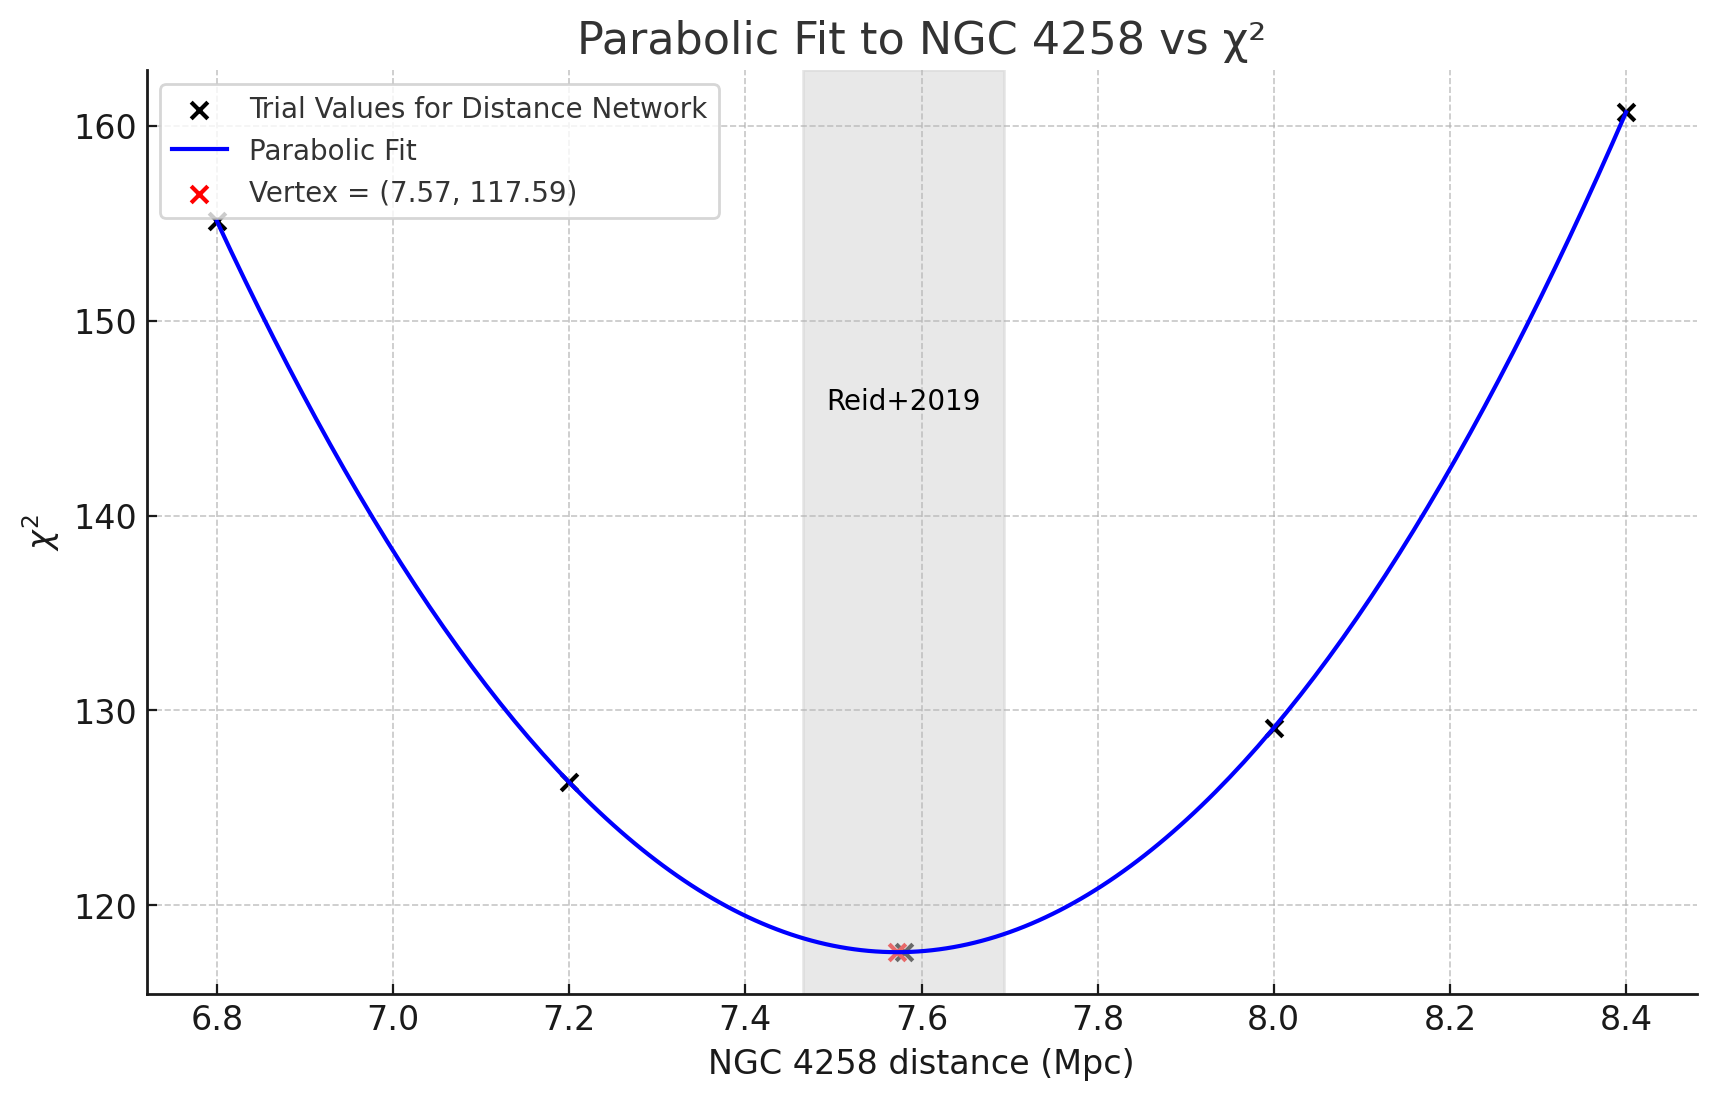
\includegraphics[width=0.95\linewidth]{Figures/N4258_trials.png}
    \caption{Trial values for the distance to NGC 4258 and associated $\chi^2$ values.  Besides the \citet{2019ApJ...886L..27R} measure at $D=7.58 \pm 0.11$ Mpc (shown as grey band) we also tried increasing or decreasing the distance by $\pm$ 5\% and 10\% (black crosses). The result its a large internal inconsistency in the distance network (due to other geometric anchors) which is highly significant. See also Table~\ref{tab:N4258_sens} for impact to $H_0$. The global minimum (vertex) is marked by a red cross.}
    \label{fig:N4258_trials.png}
\end{figure}

\begin{table}[h!]
\centering
\caption{Sensitivity of baseline to large changes in NGC 4258 distance}
\begin{tabular}{lcccc}
\hline
\textbf{Version} & \textbf{NGC 4258 Distance (Mpc)} & \textbf{$H_0$ (km s$^{-1}$ Mpc$^{-1}$)} & \textbf{Error} & \textbf{$\chi^2$} (Ndof) \\
\hline
baseline & 7.58 & 73.48 & 0.80 & 117.6 (119) \\
\hline
increased 10\% & 8.4 & 71.58 & 0.78 & 160.7 (119) \\
decreased 10\% & 6.8 & 75.43 & 0.83 & 155.1 (119) \\
increased 5\% & 8.0 & 72.53 & 0.79 & 129.1 (119) \\
decreased 5\% & 7.2 & 74.45 & 0.82 & 126.3 (119) \\
\hline
Exclude N4258 & --- & 73.08 & 0.92 & 41.7 (47)  \\
\hline
\end{tabular}
 \label{tab:N4258_sens}
\end{table}
